%%
% このファイルは、筑波大学情報学群情報メディア創成学類の
% 卒業研究論文本体のサンプルです。
% このファイルを書き換えて、この例と同じような書式の論文本体を
% LaTeXを使って作成することができます。
% 
% PC環境や、LaTeX環境の設定によっては漢字コードや改行コードを
% 変更する必要があります。
%%
\documentclass[a4paper,11pt]{jreport}

%%【PostScript, JPEG, PNG等の画像の貼り込み】
%% 利用するパッケージを選んでコメントアウトしてください。
%%
%% 推奨: graphicx パッケージ(本ファイルではこれを使用)
%%	動かない場合にいは \usepackage[dvipdfmx]{graphicx} のように dvi 変換コマンドを明示指定する。
%%
% \usepackage{graphicx} % for 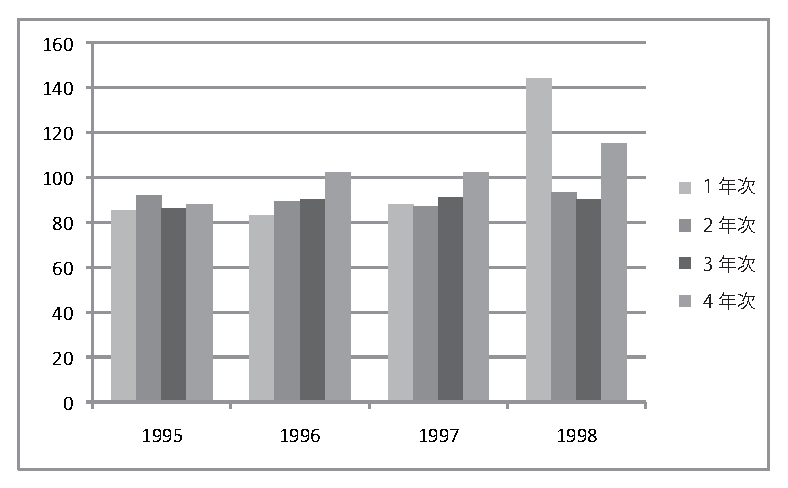
\includegraphics[width=3cm]{sample.eps}
% \usepackage[dvipdfm]{graphicx} % 画像の挿入に必要
\usepackage[dvipdfmx]{graphicx}
\usepackage[dvipdfmx]{color}
\usepackage{float} % 図の位置の強制指定に必要
%% 一応 OK (epsfig.sy)
% \usepackage{epsfig} % for 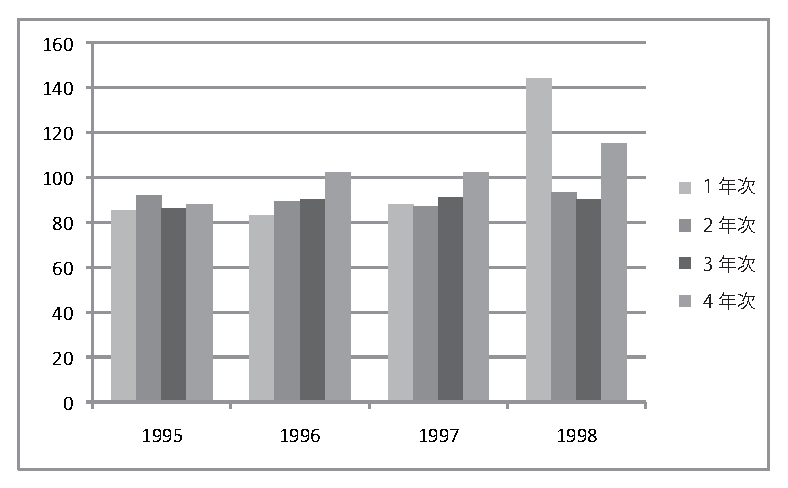
\psfig{file=sample.eps,width=3cm}
%% 以下の2つの使用はあまり勧められない (epsf.sty, epsfbox.sty)
%\usepackage{epsf} % for \epsfile{file=sample.eps,scale=0.6}
%\usepackage{epsbox} % for \epsfile{file=sample.eps,scale=0.6}

\usepackage{times} % use Times Font instead of Computer Modern
\usepackage{mdframed}
\usepackage{latexsym} % 数式で使える記号を増やす
\usepackage{amsmath} % 数式の記述環境
\usepackage{fancyhdr} % ヘッダとフッタの設定に必要
\usepackage{algorithm,algpseudocode} % 疑似コードの記述に必要
\usepackage{array}
\usepackage{booktabs} % For formal tables


\setcounter{tocdepth}{3}	% 目次を3レベル (1.2.3) まで
\setcounter{secnumdepth}{3}	% 番号付けレベル。 3: \section まで 4: \subsubsection まで
\setcounter{page}{-1}

\setlength{\oddsidemargin}{0.1in}
\setlength{\evensidemargin}{0.1in} 
\setlength{\topmargin}{0in}
\setlength{\textwidth}{6in} 
%\setlength{\textheight}{10.1in}	% ページの縦幅を変更する場合には設定する
\setlength{\parskip}{0em}
\setlength{\topsep}{0em}

%% タイトル生成用パッケージ(重要)
\usepackage{mast-jp-utf8}

%% タイトル
%% 【注意】タイトルの最後に\\ を入れるとエラーになります
\title{大規模言語モデルを用いた語用論的\\アプローチに基づく誤解可能性を考慮した\\画像情報ラベリング}
%% 著者
\author{清野 駿}
%% 指導教員
\advisor{若林 啓}

%% 年月 (提出年月)
%% 年月は必要に応じて書き替えてください。
\majorfield{ } \yearandmonth{2024年 2月}



\begin{document}
\maketitle
\thispagestyle{empty}
\newpage

\thispagestyle{empty}
\vspace*{20pt plus 1fil}
\parindent=1zw
\noindent
%%
%% 論文の概要(Abstract)
%%
\begin{center}
{\bf 概要}
\vspace{5mm}
\end{center}
本研究では,複数の画像情報が与えられたときに,そのうちの一つを誤解なく指し示すことのできる自然言語ラベルを導出する手法を提案する.

% 背景
近年,画像情報に対して適切な自然言語ラベルを付与することのできる,マルチモーダルな学習済み大規模言語モデルが広く利用可能になっている.

% 課題
しかし,大量の画像情報を一度に処理して,それぞれに特有の特徴を反映した自然言語ラベルを付与することは容易ではない.

% 研究目的
本研究では,語用論に基づく「聞き手モデル」を導入し,内省的処理を通じてラベルの品質を向上させるアプローチを提案する.

% 手法
% 大規模言語モデルを素直に用いてラベルを生成する手法をベースライン手法とし,「聞き手モデル」を導入した「強化ベースライン手法」と,単語の組み合わせによるラベル生成・改善アルゴリズムを導入した「組合せ最適化手法」の2つの提案手法によって,それぞれラベルの品質を向上させる.

% 実験
実験ではベースライン手法と2つの提案手法の計3つの手法によってラベルを生成し,これらの手法によるラベルの誤解可能性を被験者実験を通じて比較した.
%%%%%
\par
\vspace{0pt plus 1fil}
\newpage

\pagenumbering{roman} % I, II, III, IV 
\tableofcontents
\listoffigures
%\listoftables		% 本ファイルでは省略してある

%% ここから本文
\pagebreak \setcounter{page}{1}
\pagenumbering{arabic} % 1,2,3


\chapter{はじめに}

画像情報に対して自然言語のテキストを生成する技術は,様々な産業的な応用への活用が期待される \cite{Yin2023}.
特に,複数の画像が与えられたときに,それらを誤解なく指し示すことのできるテキスト表現を生成することは,ロボットによる場所のナビゲーションや,人間に対する情報提供を正確に行う上で,重要なタスクである.
本稿では,与えられた複数の画像のそれぞれに対して,それらを互いに区別可能な自然言語ラベルを生成する問題を,画像情報ラベリングと呼ぶ.

画像情報を説明する自然言語テキストを生成する手法は,画像キャプション生成の分野で研究されている \cite{Farhadi2010,Vinyals2017,Dai2023}.
特に近年では,与えられた画像情報を説明する自然言語テキストの生成や,画像情報に関する質問に回答することのできる,マルチモーダルな事前学習済み大規模言語モデルが広く利用可能になっている \cite{Gan2022}.
深層学習モデルは,モデルの規模(パラメータ数)と訓練データの規模を増加させることで品質が向上し続ける傾向があり\cite{Devlin2019},画像キャプション生成においても有効性が示されている.
このことから,可能な限り大きなスケールで事前学習した共有の大規模言語モデルを,再学習することなく活用する技術の検討が重要になってきている.

しかし,大規模言語モデルは,大量のデータをそのまま入力することはできないことから,多数のデータの関係を考慮した処理には適していない.
このため,複数の画像に対して,それらを区別する自然言語ラベルを生成する,画像情報ラベリングの問題設定における性能は十分に検証されていない.
似た画像と区別できるようなキャプションを生成する手法の研究は行われている\cite{Vedantam2017,Cohn-Gordon2018,Nie2020,Andreas2016}が,これらの研究ではキャプション生成モデルの学習を伴うことから,大規模言語モデルの性能を活用することができないという課題がある.

本研究では,画像情報ラベリングタスクにおいて,大規模言語モデルを用いたテキスト生成手法の性能を評価すると共に,語用論的アプローチに基づいて性能の向上ができるかどうかを検討する.
語用論的アプローチは,聞き手の解釈を考慮して,誤解を避けるような言語を生成するアプローチであり,複数のテキスト生成タスクにおける品質の向上が報告されている.
本研究では,2つの手法を通して,画像情報ラベリングにおける語用論的アプローチの有効性を検証する.
1つ目の手法では,大規模言語モデルに生成させた画像情報のラベルの中から,誤解の起きやすいラベルを検出し,再び大規模言語モデルに修正させる.
2つ目の手法では,大規模言語モデルに直接ラベルを生成させるのではなく,多数の特徴をテキストで挙げさせて,そのうちのいくつかを選択してラベルを構成する.
この選択においては,誤解の起きやすさを評価する聞き手モデルを内部的に持つことによって,誤解可能性を最小化するような特徴の組み合わせを発見する最適化手法を提案する.

複数の部屋の画像が与えられたときに,それぞれの部屋を指し示すラベルを生成する実験を行った.
生成したラベルの評価にはAmazon Mechanical Turkを利用し,人間がどの程度誤解するかを検証した.
実験の結果から,テキスト長が短いラベルにおいて,提案する語用論的アプローチによって性能が改善することを示す.

% 本論文では,画像に対するラベル生成における新たなアプローチを提案する.具体的には,語用論的な観点から話し手モデルと聞き手モデルを導入し,その対話を通じてラベルの改善を図る.この新たなアプローチは,生成されたラベルが画像を一意に特定できることを保証することを目的としている.また,生成したラベルの評価にはAmazon Mechanical Turkを利用し,生成されたラベルが人間にとってどの程度理解しやすいかを検証する.本論文では,提案手法とその評価結果について詳細に述べる.

% 関連研究
\chapter{関連研究}

本章では,本研究で扱う画像情報ラベリングタスクに関連する研究として,画像に基づくテキスト生成技術について\ref{sec:relwork_image_captioning}節で述べる.
また,提案手法の着想に関連する研究として,語用論的アプローチに基づく機械学習手法について\ref{sec:relwork_pragmatic_ml}節で述べる.

\section{画像に基づくテキスト生成}
\label{sec:relwork_image_captioning}
画像内容に基づくテキスト生成技術の発展は,画像キャプション生成の研究によって牽引されてきた \cite{Farhadi2010}.
特に,深層学習を用いた画像キャプション生成では,ニューラルネットワークに画像の特徴を抽出し,得られた特徴に基づいて再帰型ニューラルネットワークでテキストを生成するモデルの枠組みが用いられる \cite{Vinyals2017}.
この枠組みにおいてXuら\cite{Xu2015}は,注意機構を用いて画像内の注目すべき箇所の情報を抽出することで,生成されるキャプションの品質が向上することを示した.

一方近年,タスクによらない画像やテキストの表現学習によって,深層学習の性能が大幅に向上することが明らかになってきた \cite{Devlin2019}.
この知見を発展させて,画像とテキストのマルチモーダルモデルを構成し,これを大規模な画像とテキストのデータセットを用いて特徴量表現を学習する手法が研究されている \cite{Yin2023,Gan2022}.
事前学習済みの大規模マルチモーダルモデルを用いることで,画像キャプション生成の品質が向上する\cite{Dai2023}だけでなく,画像のゼロショット分類\cite{Radford2021}や,画像質問応答\cite{Song2022}などのタスクの精度も向上することも示されている.

さらに近年では,モデル規模と訓練データをスケールアップすることで,テキストでの指示(プロンプト)に応じた画像に基づくテキスト生成ができることが明らかになった.
Liら\cite{Li2023}は,事前訓練済みの画像特徴量抽出器とテキスト生成器の間を橋渡しするQuerying Transformerを訓練する手法によって,画像に関する自然な会話や,柔軟な指示に応じた説明の生成ができることを示した.
GPT-4\cite{Bubeck2023}は,入力した画像を描画するプログラムを出力したり,グラフの解釈もできることを示している.
例えば,「この画像の特徴を10個挙げてください」というプロンプトと共に画像を入力することで,自然言語テキストで画像の特徴を得ることができる.

これらの深層学習に基づく手法はブラックボックスであり,どこまでのタスクを実現できるかは未知数であるが,基本的には1枚あるいは少数の画像とテキストの間を結びつける処理を想定している.
このため,多数の画像に対して,それらを区別する自然言語ラベルを生成する問題設定における性能は十分に検証されていない.
本研究では,画像情報ラベリングタスクにおいて,これらのテキスト生成手法の性能を評価すると共に,画像情報ラベリングタスクを分割して再構成することによるタスク性能の向上を検討する.

\section{語用論的アプローチに基づく機械学習}
\label{sec:relwork_pragmatic_ml}
言語の生成にあたって,聞き手の解釈を考慮して,誤解を避けるような語を選ぶことは,コミュニケーションにおいて重要な要素である.
このような,話し手による聞き手の解釈を考慮したアプローチは,計算語用論と呼ばれる\cite{Fried2023}.
Rational Speech Acts (RSA)フレームワークは,計算語用論の代表的な計算モデルである \cite{Frank2012,Goodman2016}.
RSAフレームワークでは,話し手と聞き手のモデルが,それぞれ相手の目的や解釈について再帰的に推論する過程を計算する.
例えば,RSAフレームワークにおける話し手モデルは,内部的に持つ聞き手モデルに発話を解釈させたときに,伝達したい意図通りの解釈が得られるような発話を選択する.

この知見を反映して,RSAフレームワークに基づいてテキスト生成タスクの品質を向上させる手法が研究されている\cite{Fried2017}.
Williamら\cite{Williams2015}は,室内のナビゲーションタスクにおいて,計算語用論に基づく手法を提案した.
話し手モデルによって生成された複数の指示を聞き手モデルに入力し,聞き手モデルが意図通りに解釈する指示を出力する.
SAILデータセットを用いた評価により,語用論的アプローチによってナビゲーションの成功率が向上することが示された.

画像キャプション生成においても,語用論的アプローチによって,聞き手が似た画像と区別できるようなキャプションを生成する手法が提案されている\cite{Vedantam2017,Cohn-Gordon2018,Nie2020}.
Andreasら\cite{Andreas2016}は,画像の参照ゲームにおいて,聞き手の誤解を低減するようなキャプションを生成する手法を提案した.
これらの手法は,ニューラルネットワークでモデル化された話し手と聞き手の学習を伴うことから,近年極めて高い品質を達成している大規模事前学習済みモデルを活用することが難しい.
本研究では,大規模事前学習済みモデルを再学習することなく用いる語用論的アプローチによって,誤解可能性を考慮した画像情報ラベリングを実現する手法を検討する.

%提案手法
\chapter{提案手法}

\section{問題設定}

本研究では,画像の集合が入力されたときに,それぞれの画像を,人が一意に誤解なく特定できるラベルを生成する問題に取り組む.

n枚の画像の集合を\(X = \{x_1, x_2, \ldots, x_n\}\)とする.\(X\)に対して付与されるラベルの集合を\(Y = \{y_1, y_2, \ldots, y_n\}\)とする.ラベル\(y_1, y_2, \ldots, y_n\)は画像\(x_1, x_2, \ldots, x_n\)にそれぞれ対応しており,各ラベルは対応する画像の特徴を説明するものとする.

ここで,ラベル\(y_r\)($r \in [1..n]$)と\(X\)を被験者に与えたとき,被験者が\(y_r\)に対応する画像\(x_r\)を選択しようとして,\(x_r\)以外を選択してしまう確率を誤解可能性\(p\)とする.

提案手法では,\(p\)が最小となるラベルの組み合わせ\(Y\)を生成することを目的とする.


\section{話し手モデルと聞き手モデル}

本研究の手法では,語用論的アプローチに基づき問題解決を図る.

語用論とは,話し手と聞き手が互いの意図を理解する過程を研究する学問であり,皮肉表現や比喩表現などを研究対象とする.

本研究での語用論的アプローチは,話し手モデルと聞き手モデルの対話を通じて,問題への回答を改善していく.

話し手モデルは,画像を詳細かつ正確に説明するラベルを生成することに重点を置く.この過程では,画像の特徴や意味内容を考慮し,誤解を引き起こす可能性のある曖昧な表現を避けることが重要である.一方,聞き手モデルは,生成されたラベルがどの程度誤解を招く可能性があるかを評価する.このモデルは,ラベルが提供する情報が明確で,かつ他のラベルとの誤解が起きないかどうかを評価し,話し手モデルに対してフィードバックを行う.
\subsection{話し手モデルと聞き手モデルの役割}

\begin{itemize}
  \item 話し手モデル:画像を説明するラベルを生成し,その改善を行う.
  \item 聞き手モデル:生成されたラベルに対する誤解可能性を評価し,各画像を誤解なく選択できるかを判断する.
\end{itemize}


% \section{ベースライン(ChatGPT手法)}
% プロンプトの説明中心
\section{Pragmatic ChatGPT(PCG)手法}

PCGでは,話し手モデルと聞き手モデルの両方をChatGPTを用いて実装し,ラベル生成を行う.

この手法では,以下のステップでラベルを生成し,繰り返し改善を図る.このステップでは,1,3が話し手モデル,2が聞き手モデルの役割を担っている.

\begin{enumerate}
  \item ChatGPTに対して画像の集合Xを入力する.Xに含まれる各画像に対して,それぞれ誤解なく画像を区別できるラベルを出力するように,プロンプトを入力する.ここで出力されたラベルの集合をY1とする.
  \item ラベルの集合Y1と画像の集合XをChatGPTに入力する.Y1に含まれる各ラベルについて誤解可能性を分析し,ラベル改善のヒントを出力するように,プロンプトを入力する.出力されたラベル改善のヒントをH1とする.
  \item ChatGPTに対して画像の集合X,ラベル改善のヒントH1,ラベルの集合Y1を入力する.H1を参考にして,Y1を改善した新たなラベルを出力するように,プロンプトを入力する.ここで出力されたラベルの集合をY2とする.
  \item 2と3を繰り返して,最終的に得られたラベルの集合Ym(mは任意の自然数)を,誤解可能性の低いラベルとして提出する.
\end{enumerate}

各モデルごとに行っている処理を以下に示す.

\begin{itemize}
  \item 話し手モデル(生成モデル)
    \begin{itemize}
      \item 初期ラベル生成:Xに含まれる各画像に対応するラベルY1を出力する.
      \item 改善ラベル生成:聞き手モデルによって出力されたヒントHと,X,Y1から,Y1を改善したラベルY2を出力する.
    \end{itemize}
  \item 聞き手モデル
    \begin{itemize}
      \item ヒント生成:XとY1から,ラベル改善のヒントHを出力する
    \end{itemize}
\end{itemize}

なお,出力するラベルの長さに制限をかける場合は,ラベル出力処理を行っている部分のプロンプトに以下を追加する.この例では10単語以内でラベルを出力するように指定している.

\begin{figure}[H]
	\begin{mdframed}[linewidth=1pt]
	Tray ceiling Recessed lighting, Beige wall paint, ..., Decorative straw hats on wall, Distressed wood mirror frame
	\end{mdframed}
	\caption{プロンプトの例}
	\label{fig:baseline_prompt}
\end{figure}
	
% プロンプトとその組み合わせ,サイクルの説明

\section{特徴量に基づく組み合わせ最適化手法}
\subsection{全体の流れ}
特徴量に基づく組合せ最適化手法(FCO)では,画像から特徴を表す単語群を生成し,これを基に最適なラベルを導き出していく.このプロセスは,話し手モデルと聞き手モデルの相互作用によって実現される.
以上の処理の流れをまとめた図を図\ref{fig:cof_flow_example}に示す.

\begin{figure}[H]
  \centering
  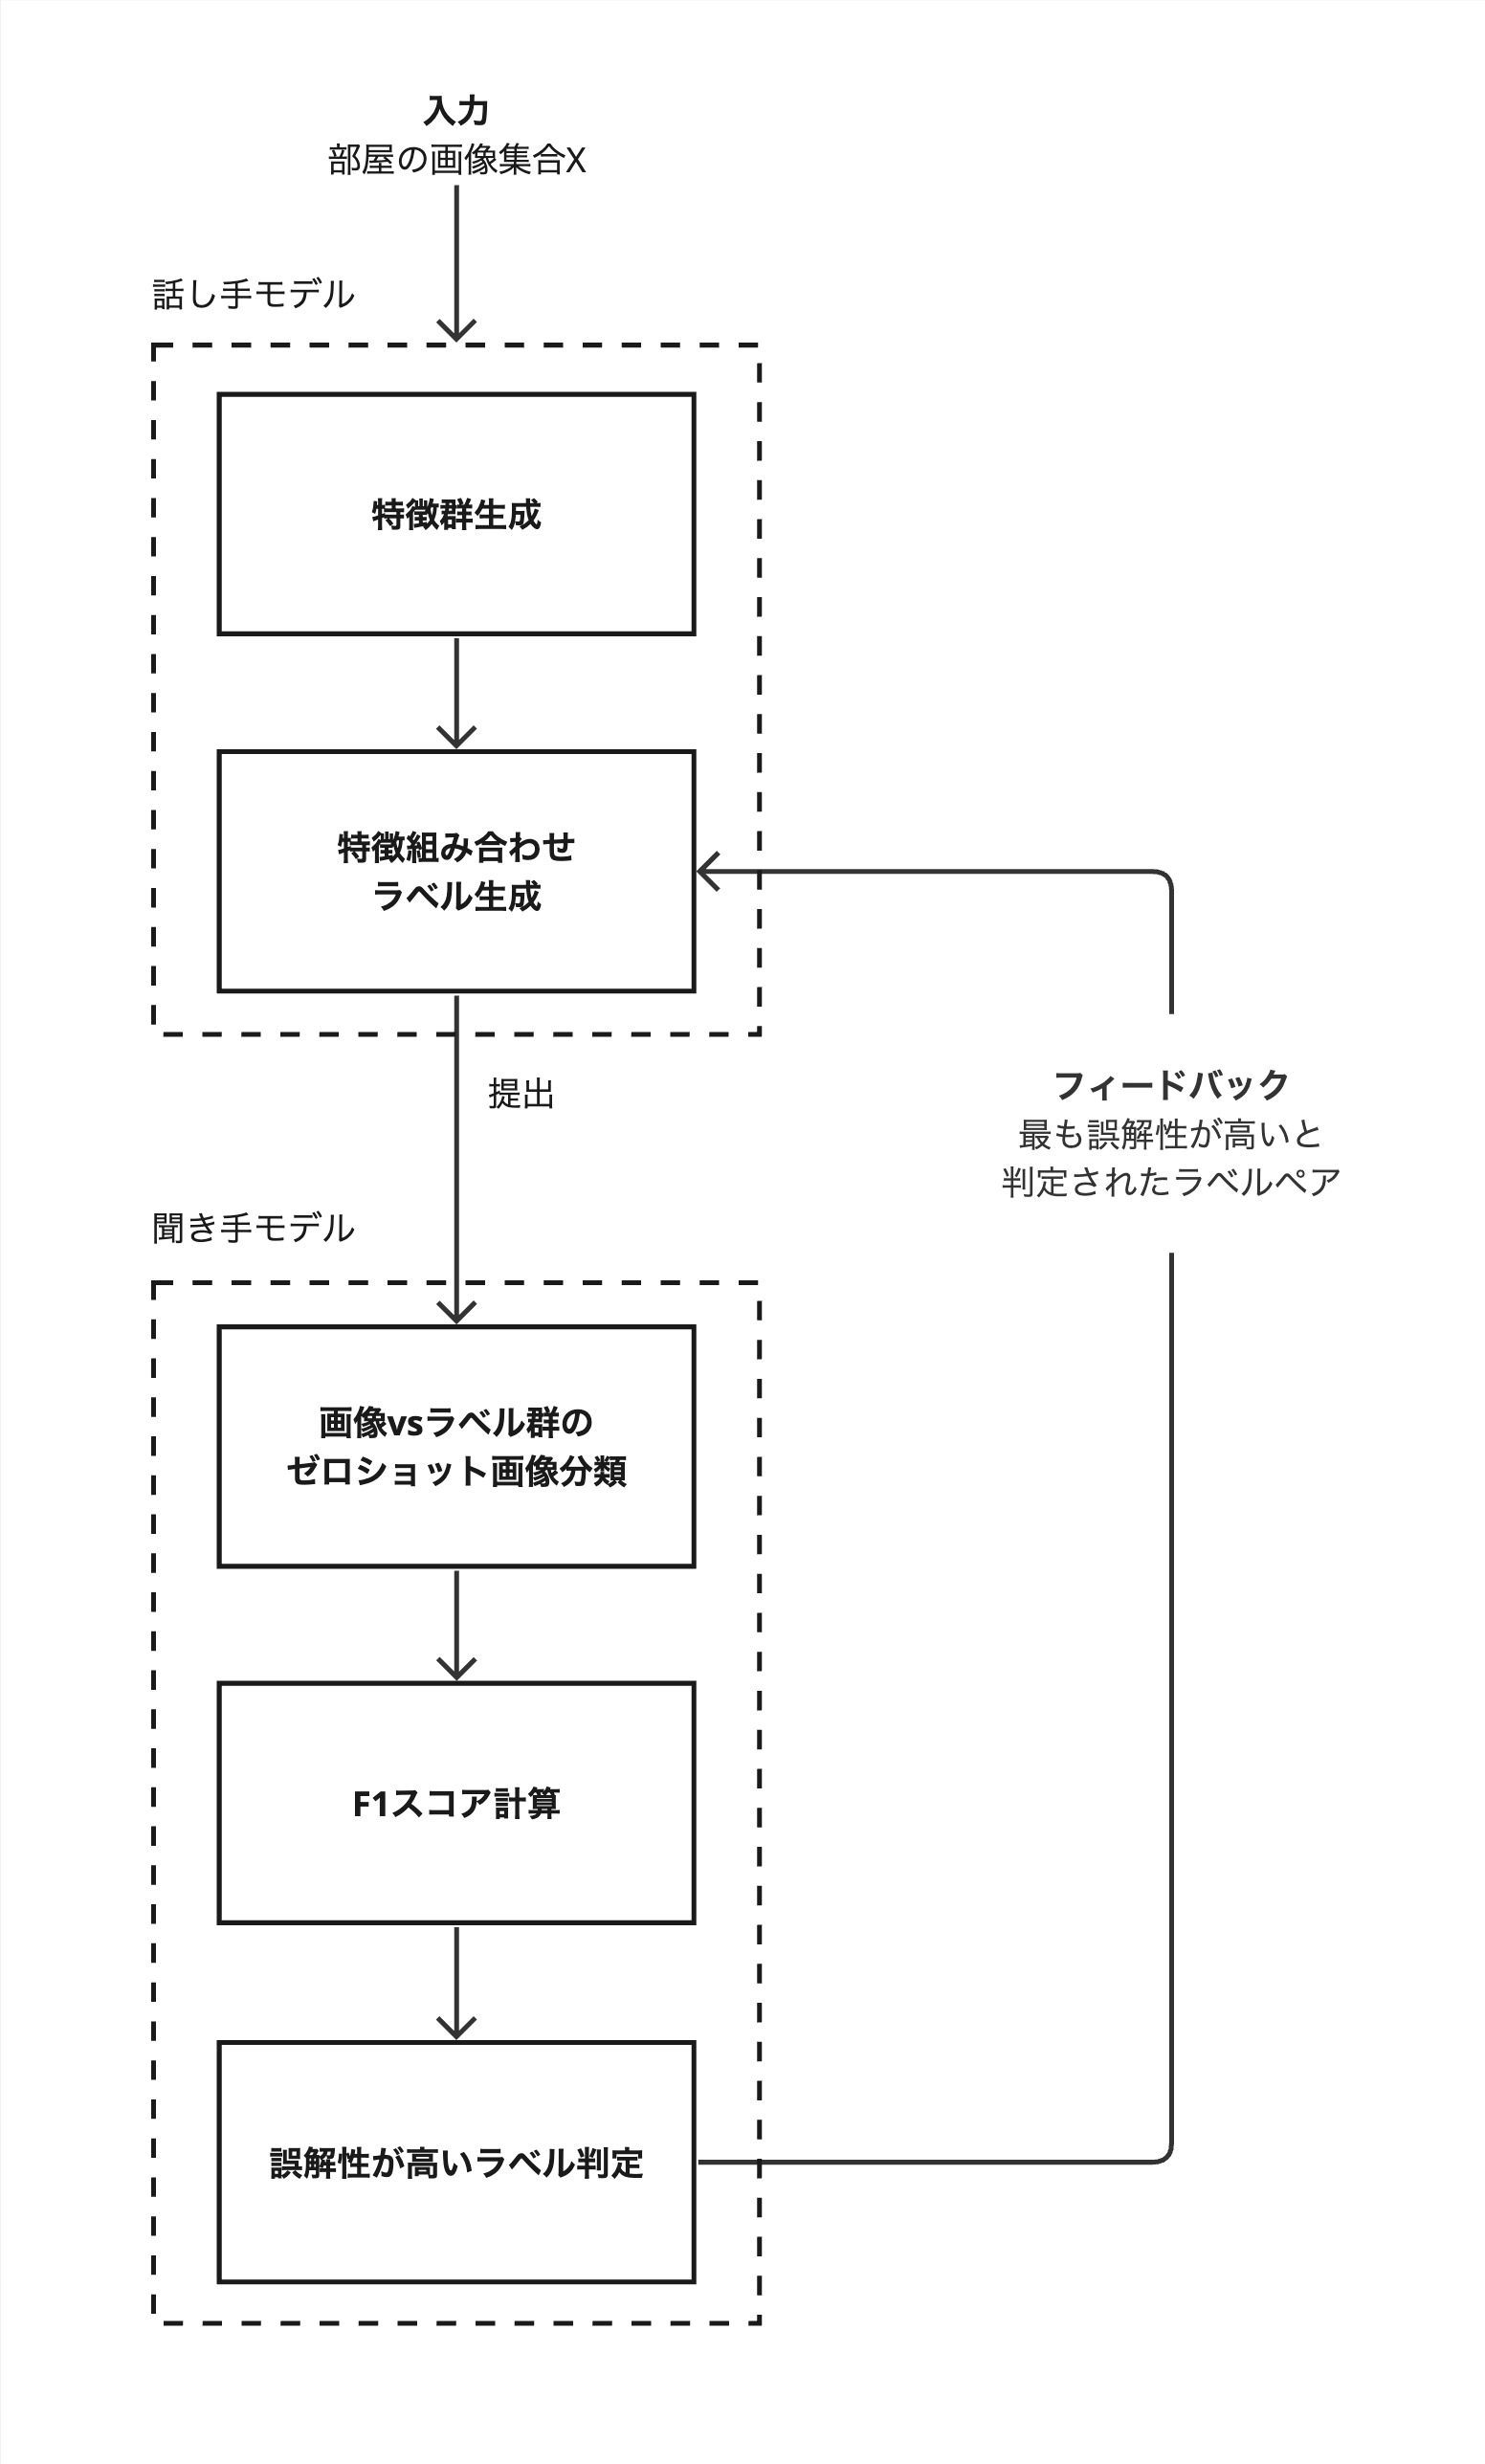
\includegraphics[width=3.5in]{figures/COF_flow.jpg}
  \caption{ラベル生成の流れ}
  \label{fig:cof_flow_example}
\end{figure}

\subsection{特徴群生成とラベル生成}
初めに,話し手モデル(ChatGPT-4)に画像群$X$を入力し,各画像から特徴を表す単語群$Z$を生成する.特徴群$Z$の例は図\ref{fig:feature_group}に示す.この際,各画像からは50個の特徴$z$が得られる.次に,これらの特徴群$Z$からランダムに特徴を選び,組み合わせてラベル$y$を生成する.これを画像群$X$全体で行い,ラベル集合$Y_1$を作成する.

\begin{figure}[H]
\begin{mdframed}[linewidth=1pt]
Tray ceiling Recessed lighting, Beige wall paint, ..., Decorative straw hats on wall, Distressed wood mirror frame
\end{mdframed}
\caption{部屋X1の特徴群Z1}
\label{fig:feature_group}
\end{figure}

続いて,聞き手モデルに$Y_1$と$X$を入力する.このモデルは,各ラベルの誤解可能性を分析し,最も誤解性が高いラベル組をヒント$H_1$として出力する.
\subsection{ゼロショット画像分類}
生成されたラベルの誤解可能性を評価するため,ゼロショット画像分類を実施する.このプロセスでは,生成されたラベル群$Y_1$と単一の画像$x_1$を入力として与える.ゼロショット画像分類を適用し,画像$x_1$が各ラベルに属する確率を確率分布として出力する.
この手順は画像$x_1$から$x_n$に至るまで同様に行われる.
実際にゼロショット分類をした際の結果を図\ref{fig:zeroshot_result}に示す.
\begin{figure}[H]
  \centering
  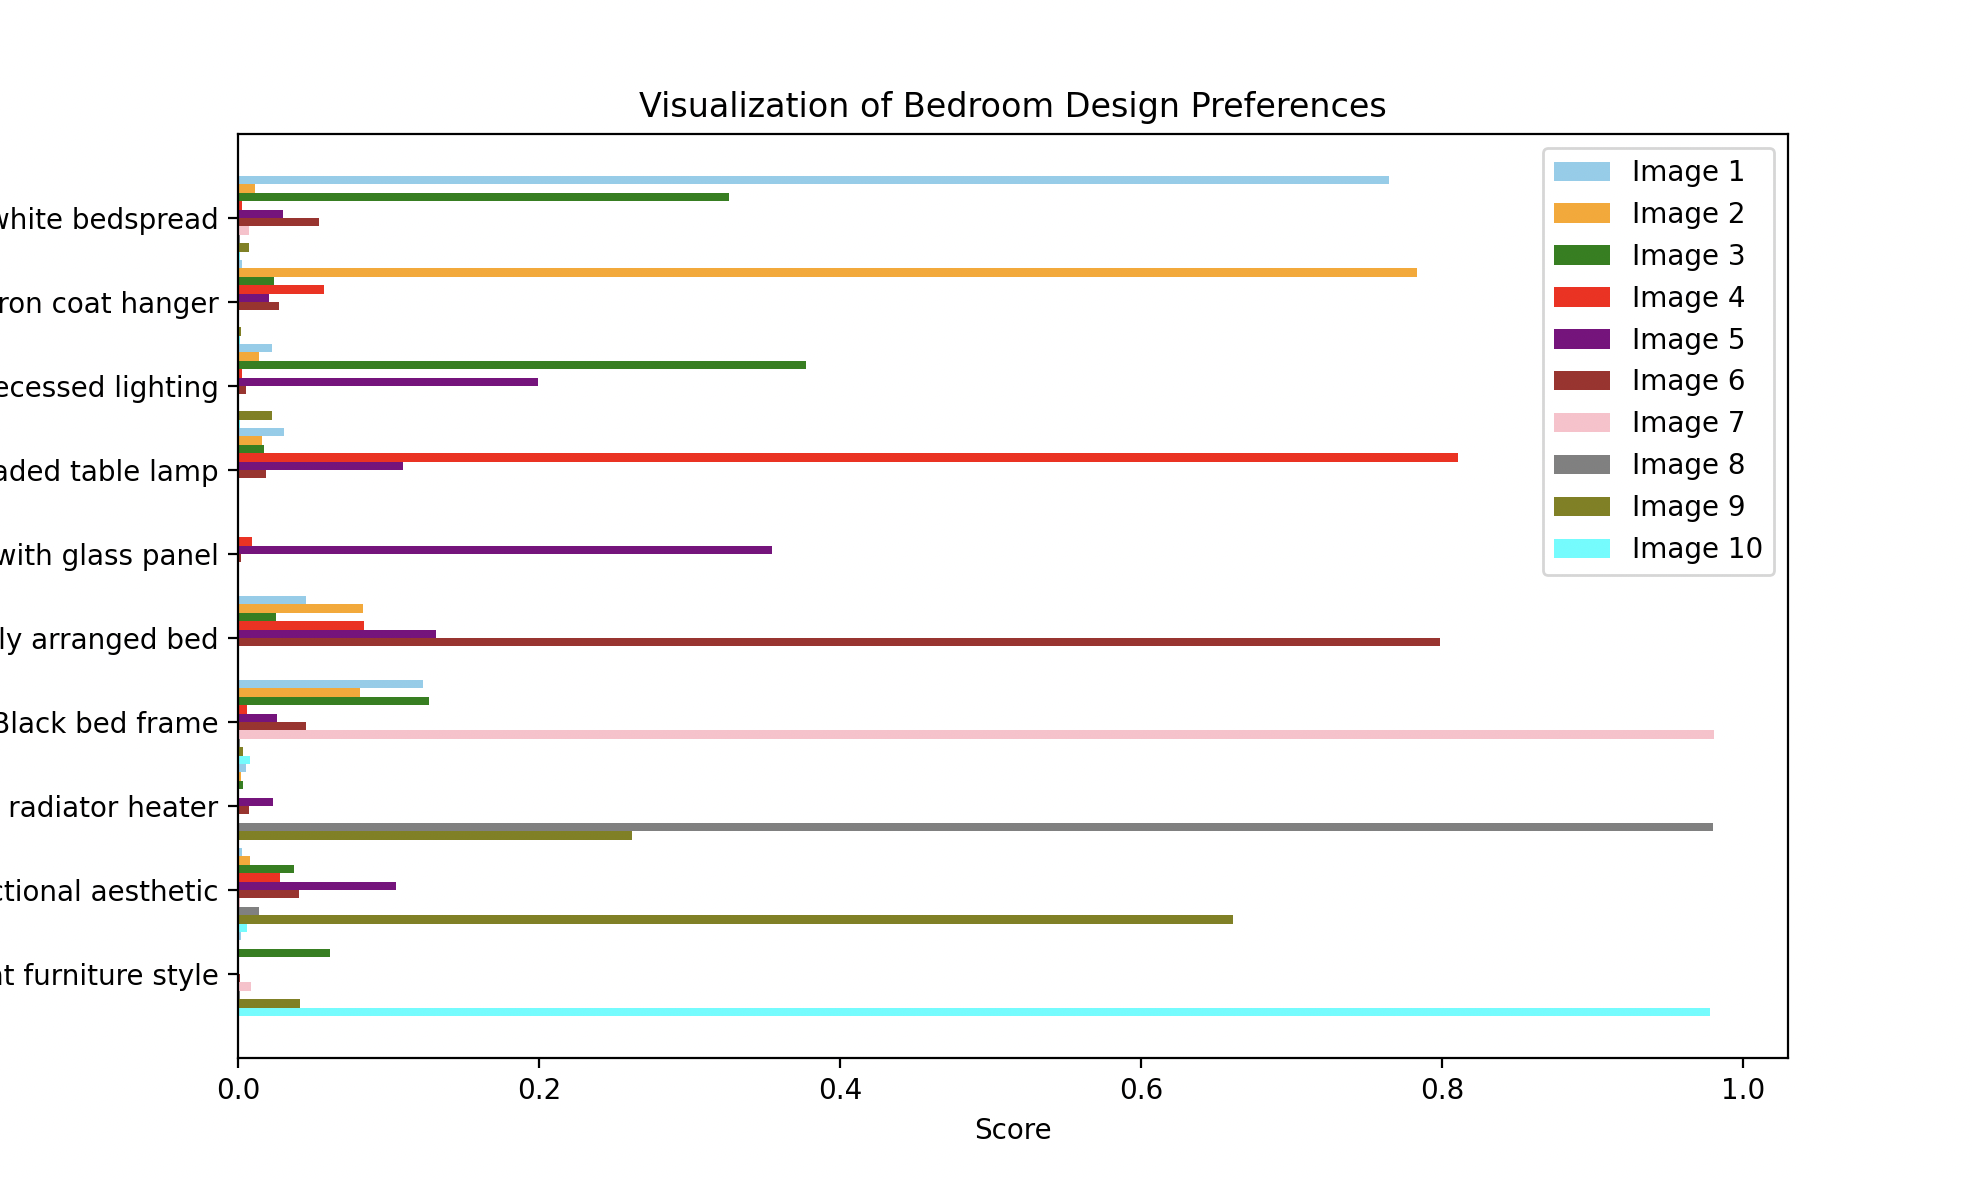
\includegraphics[width=\linewidth]{figures/zeroshot_result.png}
  \caption{ゼロショット分類の結果}
  \label{fig:zeroshot_result}
\end{figure}
\subsection{F1スコア計算}
ラベルセットの誤解可能性はゼロショット画像分類の結果を用いて計算されたF1スコアで評価される.
ゼロショット画像分類を行ったときに,$i$番目の画像に対して,$j$番目のラベルに与えられた確率を$p_{i,j}$とすると,ラベル$j$の適合率は$\frac{p_{j,j}}{\sum_i(p_{i,j})}$,再現率は$p_{j,j}$である.

ラベル$j$のF1スコアは,ラベル$j$の適合率と再現率の調和平均で求められる.そして全ラベル$Y$に対してそれぞれF1スコアを求め,全F1スコアの平均をラベルの性能とする.
\subsection{誤解性の高いラベルペア判定}
ゼロショット画像分類の結果を分析して改善すべきラベルのペアを特定する過程では,画像$x_k$を説明したラベル$y_k$とし,$x_k$以外の画像の中で$y_k$への所属確率が最も高いものを$y_1$から$y_n$で取得する.自分の画像以外の画像の所属確率が最も高いラベルと,最も高い画像の真の正解ラベルを改善ペアとして出力する.このペアは,ゼロショット分類において最も誤解されやすい,つまり最も性能が低いと判断されるラベルと,そのラベルが誤って関連付けられた画像の正しいラベルである.
\subsection{聞き手モデルから受け取ったヒントをもとにラベルを改善}
次に,話し手モデルに$H_1$を入力し,$Y_1$を改善した新たなラベル集合$Y_2$を生成する.この際,画像とテキストのペアを大規模に学習することで,画像の内容を説明するテキストとの類似度を計算できるモデルであるCLIP(Contrastive Language–Image Pre-training)を使用する.CLIPは,画像とテキストの両方を同じ空間に埋め込むことで,その類似度を測定する.ここでの類似度は画像とラベルの特徴の重要度として扱う.各特徴と画像との重要度の例は表\ref{tab:similarity_examples}に示す.

\begin{table}[ht]
\centering
\caption{各特徴と画像との重要度の具体例}
\label{tab:similarity_examples}
\begin{tabular}{@{}lr@{}}
\toprule
特徴 & 重要度 \\ \midrule
Tray ceiling Recessed lighting & 28.051437 \\
Two-tone wood flooring & 25.21447 \\
White ceiling & 25.036436 \\
\addlinespace % Adds some space before the dots
\multicolumn{2}{c}{\dots} \\ % Centered dots to indicate omitted data
\addlinespace % Adds some space after the dots
Mountainous landscape view & 17.63242 \\
Glass vase with white flowers & 17.470116 \\
Striped throw on the bed & 16.694729 \\ \bottomrule
\end{tabular}
\end{table}


与えられた改善すべき2つのラベルセット(\texttt{current\_label1}と\texttt{current\_label2})に対して,それぞれのラベルセットが表す画像(\texttt{image1}と\texttt{image2})との重要度を参考にしながら改善する処理を行う.以下にその処理をステップごとに説明する.

\begin{enumerate}
    \item \textbf{current\_label1 vs image1}\\
    \texttt{current\_label1}の中から,\texttt{image1}との類似度が最も低いラベルを確率的に選択.これは,類似度の逆数をソフトマックス関数にかけることで確率分布を作成し,その分布に基づいてランダムに選択することで行う.
    \item \textbf{all\_label1 vs image1}\\
    \texttt{all\_label1}の中から\texttt{current\_label1}に含まれていないラベルを対象に,\texttt{image1}との類似度が高いラベルから確率的に選択する.
    \item \textbf{current\_label1 vs image2}\\
    \texttt{current\_label1}の中から,\texttt{image2}との類似度が高いラベルを確率的に選択.これは,類似度をソフトマックス関数にかけることで確率分布を作成し,その分布に基づいてランダムに選択することで行う.
    \item \textbf{all\_label1 vs image2}\\
    \texttt{all\_label1}の中から\texttt{current\_label1}に含まれていないラベルを対象に,\texttt{image2}との類似度が低いラベルを確率的に選択する.
    \item \textbf{ラベルの入れ替え}\\
    \texttt{current\_label1}からステップ1で選んだラベルとステップ4で選んだラベルを除外し,ステップ2と3で選んだラベルを追加して新しいラベルセット\texttt{new\_label1}を作成する.
    \item \textbf{重複の削除}\\
    最後に,\texttt{new\_label1}と\texttt{new\_label2}から重複しているラベルを削除する.これにより,各ラベルセットがユニークなラベルのみを含むようになる.
    \item \textbf{curent\_label2でも同様の処理をしてnew\_label2を作成する.}
    \item \textbf{改善されたラベルセットの返却}\\
    処理を経て改善された\texttt{new\_label1}と\texttt{new\_label2}を関数の出力として返却する.
\end{enumerate}
これにより,\texttt{current\_label1}と\texttt{current\_label2}はそれぞれの画像に対する識別性が改善され,画像とラベルの関連性が高まるように調整される.
このプロセスを繰り返し,ラベル集合$Y_m$を誤解可能性が低くなるように改善していく.
最終的に,全試行の中で最も平均F1スコアが高い時のラベル組み合わせを出力する.
全試行内の平均F1スコアが以下の図\ref{fig:f1_score}の場合,赤丸の時のラベルセットを最終的な出力とする.
\begin{figure}[H]
  \centering
  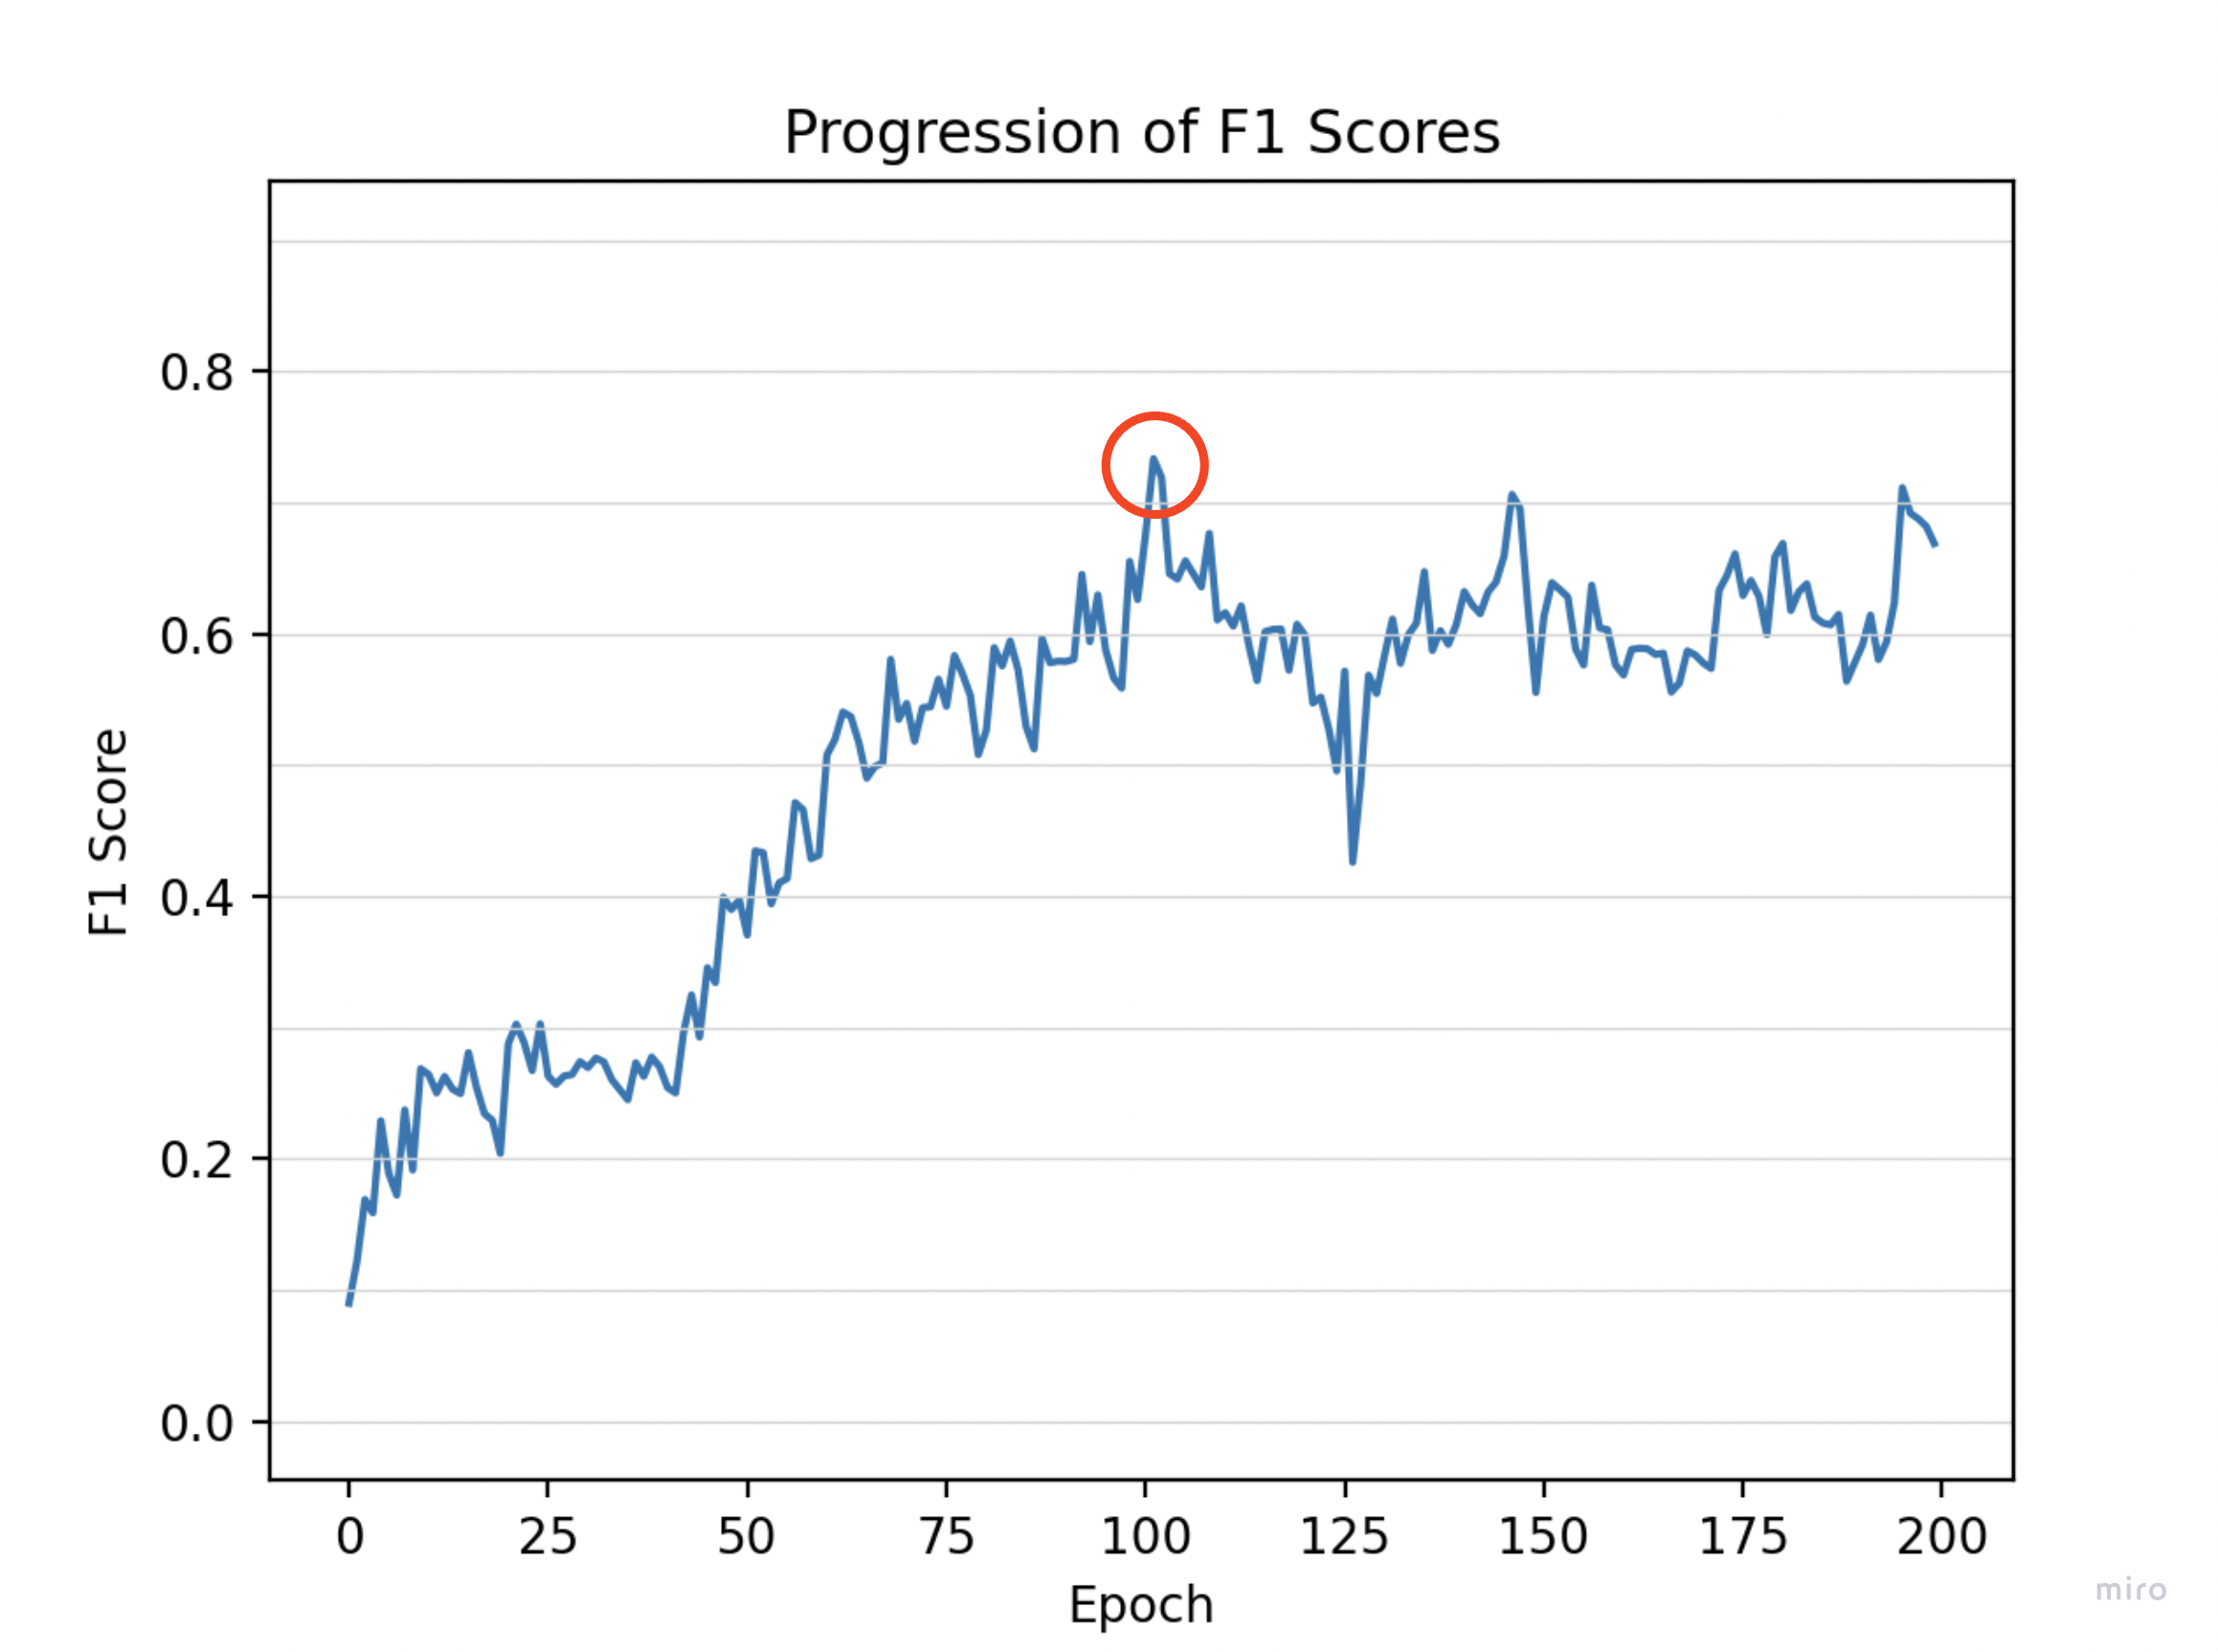
\includegraphics[width=\linewidth]{figures/f1_score.png}
  \caption{200回試行内のF1スコアの推移}
  \label{fig:f1_score}
\end{figure}
この手法では,話し手モデルが特徴群の生成,特徴の組み合わせによるラベル生成,ヒントに基づくラベルの改善を担い,聞き手モデルが各画像の選択の正確性評価,ラベルの誤解可能性の分析,改善すべきラベル組のヒント出力を行う.この相互作用により,画像に対する最適なラベルを効果的に生成することを試みる.

\section{特徴量に基づく組み合わせ最適化手法(New)}
本節では,LLMに直接ラベルを生成させるのではなく,画像情報の特徴を列挙させ,そのうちのいくつかを選択してラベルを構成する提案手法について述べる.
提案手法は,聞き手がラベルを解釈し,指し示している画像の候補を絞り込む過程を明示的に考慮する.

画像 $x_i$ に対して,特徴量 $Z_i = \{z_1, \ldots, z_m\}$ を生成させる.$m$ は1枚の画像情報あたりの特徴量の数である.例えば,図xの部屋であれば,$z_1 = \text{'red bed'}$, $z_2 = \text{'...'}$ など


\chapter{形式}

ここでは、論文の表紙および本体の記述方法について述べる。

\section{表紙}

表紙は、{\tt $\backslash$maketitle} によって作成するため、
以下の項目に相当する文字列をそれぞれ記述する。

\begin{description} \parskip=1pt
\item{題目: }
	題目は{\tt $\backslash$title} に記述する。
	行替えを行う場合は$\backslash\backslash$ を入力する。
	ただし、題目の最後に$\backslash\backslash$ を入力するとコンパイルが通らなくなるので注意する。
	なお、4行以上の題目の場合、表紙ページがあふれるためスタイルファイル``mast-jp-xxx.sty''を変更する必要がある
	(xxx は使用文字コードに合わせて euc, sjis, utf8 のいずれかになる)。
\item{著者名: }
	著者名は{\tt $\backslash$author} に記述する。
\item{指導教員名: }
	指導教教員は{\tt $\backslash$advisor} に記述する。
\item{年月: }
	年月は{\tt $\backslash$yearandmonth} に記述する。
	\\
	年月は別途指示された場合はそれにしたがう(指示がなければ提出時のものを記述する)。
\end{description}

\section{本体}

本体は1段組で記述する。

図表には番号と説明(caption)を付け、文章中で参照する。
表 \ref{table:fundamental_data_type}と図\ref{figure:sample} は
それぞれ表と図の例である。
表の説明は上に、図の説明は下に書くことが多い。
図の挿入に用いるパッケージについては使用環境に合わせて自由に選択してほしい。

\begin{table}[hbt]
\caption{表の例}
\label{table:fundamental_data_type}
\begin{center}
\begin{tabular}{| c | r | r | r | r |}
\hline
年 度 & 1年次 & 2年次 & 3年次 & 4年次 \\
\hline
1995 & 85 & 92 & 86 & 88 \\
1996 & 83 & 89 & 90 & 102 \\
1997 & 88 & 87 & 91 & 112 \\
1998 & 144 & 93 & 90 & 115 \\
\hline 
\end{tabular}
\end{center}
\end{table}
\medskip

\begin{figure}[htbp]
\begin{center}
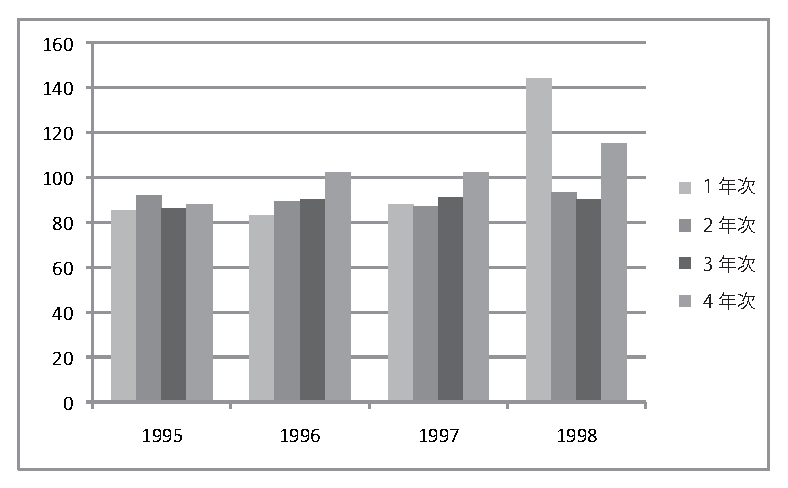
\includegraphics[scale=0.6]{sample.eps}
%% epsfig.sty を使う場合には上の行を次のように変更する
% 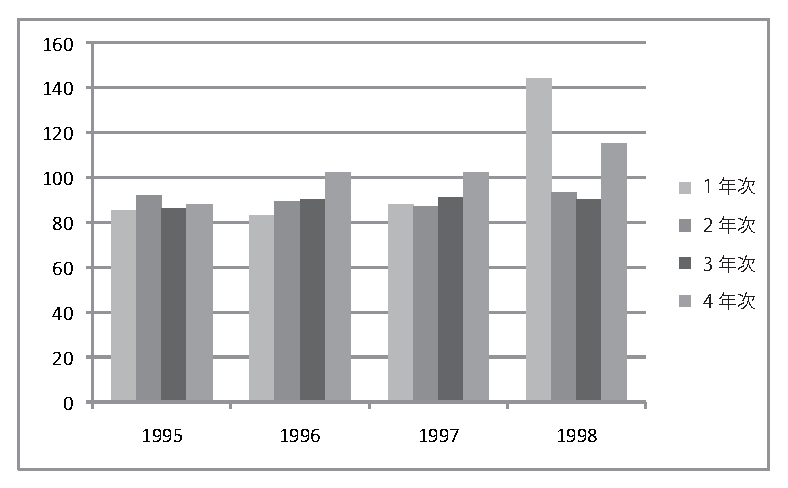
\psfig{file=sample.eps,scale=0.6}
\end{center}
\caption{図の例 (graphicx パッケージを使用)}
\label{figure:sample}
\end{figure}

詳しくは参考書\cite{okumura2010,yoshinaga2009}などを参照のこと。
奥村晴彦氏の「\TeX Wiki」 https://texwiki.texjp.org/ は
日本語の\TeX に関する情報が充実している。
具体的な文献の参照例として
本の例\cite{ware2004}、
雑誌論文の例\cite{meyer2009}、
予稿集の例\cite{hill2010}
を挙げておく。

\chapter*{謝辞}
\addcontentsline{toc}{chapter}{\numberline{}謝辞}	% 目次で左詰めするなら \numberline{} を削除する。

必須ではないが、書くことが望ましい。
\\
研究補助を受けている場合、他に指定がなければここに書く。

\newpage

\addcontentsline{toc}{chapter}{\numberline{}参考文献}	% 目次で左詰めするなら \numberline{} を削除する。
\renewcommand{\bibname}{参考文献}

%% 参考文献に jbibtex を使う場合
%\bibliographystyle{junsrt}
%\bibliography{samplebib}
%% [compile] jbibtex sample; platex sample; platex sample;
% 参考文献
\bibliographystyle{junsrt}
\bibliography{reference}
%% 参考文献を直接ファイルに含めて書く場合
% \begin{thebibliography}{99}
% \bibitem{okumura2010}
% 奥村晴彦: 
% LaTeX2e美文書作成入門 改訂第5版, 
% 技術評論社, 2010年.	% 「年」の字はなくてもよい。

% \bibitem{yoshinaga2009}
% 吉永徹美: 
% LaTeX2$\varepsilon$辞典, 
% 翔泳社, 2009年.		% 「年」の字はなくてもよい。

% \bibitem{ware2004} 
% Colin Ware:
% Information Visualization --- Perception for Design (Second Edition), 
% Morgan Kaufmann Publishers, 486~pp., 2004.
% %% 本のタイトルはイタリックにする流儀もある。その場合には全体を {\it ... } で囲む。
% %% 氏名の途中で改行させないためには、Colin~Ware のようにハードスペースを入れる。

% \bibitem{meyer2009}
% Miriah Meyer and Tamara Munzner:
% MizBee: A Multiscale Synteny Browser, 
% {\it IEEE Transactions on Visualization and Computer Graphics},
% Vol.~15, No.~6, pp.~897--904, 2009.

% \bibitem{hill2010}
% Emerson Murphy-Hill and Andrew P. Plack: 
% An Interactive Ambient Visualization for Code Smells, 
% {\it in Proceedings of the 2010 International Symposium on Software Visualization (SOFTVIS' 10)},
% pp.~5--14, 2010.

% \end{thebibliography}

\end{document}
